\documentclass{article}
\usepackage{amsmath}
\usepackage{tikz}

\begin{document}

The jumps of $\boldsymbol{M}(z)$. Recall, $\boldsymbol{L}_{k}$ and $\boldsymbol{U}_k$ are defined in equation \eqref{notationDefs}.

\begin{figure}[h]
    \centering
    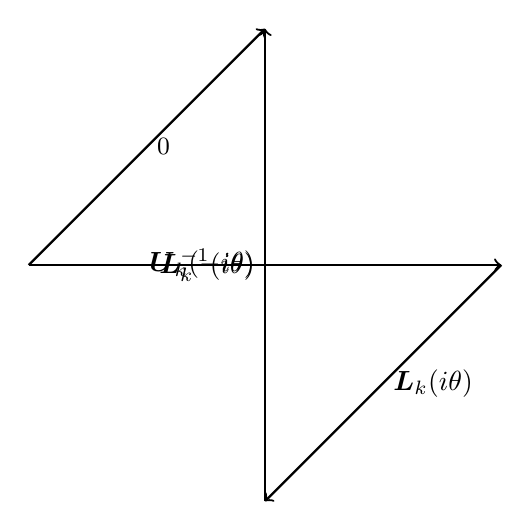
\begin{tikzpicture}[scale=1.5]
        % Define coordinates
        \coordinate (A) at (-2, 0);
        \coordinate (B) at (2, 0);
        \coordinate (C) at (0, -2);
        \coordinate (D) at (0, 2);
        
        % Draw arrows and labels
        \draw[->,thick] (A) -- node[left] {$\boldsymbol{L}_{k}^{-1}(i\theta)$} (B);
        \draw[->,thick] (C) -- node[left] {$\boldsymbol{U}_{k}(-i\theta)$} (D);
        \draw[->,thick] (A) -- node[right] {\small $0$} (D);
        \draw[->,thick] (B) -- node[right] {$\boldsymbol{L}_{k}(i\theta)$} (C);
    \end{tikzpicture}
    \caption{Illustration of the jumps of $\boldsymbol{M}(z)$.}
    \label{fig:jumpsOfM}
\end{figure}

\end{document}